% questions.tex —— 2006 年·普通高考·安徽卷理科 · 题目内容片段（无答案）
% 由 tools/generate_projects.py 依来源总账自 2006/2006_数学真题_安徽理_试题.md 生成，勿手改（改源 MD 后重跑）


\begin{gktip}
\textbf{来源及状态}：依据本机固定 PDF 第 1–2 页转录。固定文件 SHA-256 与 source manifest 中对应记录一致。首页题签自题“2006 普通高等学校招生考试（安徽卷理）”，印刷页码为 276–277；这只能确认固定副本的字节和页内可见文字，不能证明 PDF 的发布者、出版社、版次、来源链或官方原件身份。固定副本没有答案、解析或评分页。

\textbf{源页定位}：PDF 第 1 页（印刷页码 276）含第 1–18 题：左栏第 1–7 题，中栏第 8–16 题，右栏第 17–18 题；PDF 第 2 页（印刷页码 277）含第 19–22 题。题图位于第 1 页 Q6、Q16，以及第 2 页 Q19、Q22。

\textbf{待核}：Q3 的椭圆式在固定副本中只见 $\dfrac{x^2}{6}+\dfrac{y^2}{2}$，其后直接接“的右焦点”，未见等号及右侧；本稿照录可见内容，不据常见方程形式补写。
\end{gktip}

\gkpart{一、选择题}

\begin{question}
\gkti{1}复数 $\dfrac{1+\sqrt{3}i}{\sqrt{3}-i}$ 等于\mbox{（　　）}

（A）$i$　（B）$-i$　（C）$\sqrt{3}+i$　（D）$\sqrt{3}-i$

\end{question}
\begin{question}
\gkti{2}设集合 $A=\{x\mid |x-2|\leqslant 2,\ x\in\mathbb R\}$，$B=\{y\mid y=-x^2,\ -1\leqslant x\leqslant 2\}$，则 $\complement_{\mathbb R}(A\cap B)$ 等于\mbox{（　　）}

（A）$\mathbb R$　（B）$\{x\mid x\in\mathbb R,\ x\ne0\}$

（C）$\{0\}$　（D）$\varnothing$

\end{question}
\begin{question}
\gkti{3}若抛物线 $y^2=2px$ 的焦点与椭圆 $\dfrac{x^2}{6}+\dfrac{y^2}{2}$ 的右焦点重合，则 $p$ 的值为\mbox{（　　）}

\begin{gktip}
待核：固定副本只见上述椭圆式，未见等号及右侧；按固定副本照录。
\end{gktip}

（A）$-2$　（B）$2$　（C）$-4$　（D）$4$

\end{question}
\begin{question}
\gkti{4}设 $a,b\in\mathbb R$，已知命题 $p\text{：}a=b$；命题 $q\text{：}\left(\dfrac{a+b}{2}\right)^2\leqslant\dfrac{a^2+b^2}{2}$，则 $p$ 是 $q$ 成立的\mbox{（　　）}

（A）必要不充分条件　（B）充分不必要条件

（C）充分必要条件　（D）既不充分也不必要条件

\end{question}
\begin{question}
\gkti{5}函数
\nopagebreak[4]
\[
y=\begin{cases}
2x,&x\geqslant0,\\
-x^2,&x<0,
\end{cases}
\]
的反函数是\mbox{（　　）}

（A）$y=\begin{cases}\dfrac{x}{2},&x\geqslant0,\\\sqrt{-x},&x<0\end{cases}$　（B）$y=\begin{cases}2x,&x\geqslant0,\\\sqrt{-x},&x<0\end{cases}$

（C）$y=\begin{cases}\dfrac{x}{2},&x\geqslant0,\\-\sqrt{-x},&x<0\end{cases}$　（D）$y=\begin{cases}2x,&x\geqslant0,\\-\sqrt{-x},&x<0\end{cases}$

\Needspace{0.4\textheight}
\end{question}
\begin{question}
\gkti{6}将函数 $y=\sin\omega x$（$\omega>0$）的图象按向量 $\vec a=\left(-\dfrac{\pi}{6},0\right)$ 平移，平移后的图象如图所示，则平移后的图象所对应的函数解析式是\mbox{（　　）}
\nopagebreak[4]
\begin{center}% 2006 安徽卷理 Q6；依固定源页重绘坐标轴、正弦曲线和标注。
\begin{tikzpicture}[x=1.45cm,y=0.95cm,line cap=round,line join=round,>=stealth,font=\small]
  \draw[->] (-0.9,0) -- (3.4,0) node[right] {$x$};
  \draw[->] (0,-1.5) -- (0,1.65) node[above] {$y$};
  \draw[thick,domain=-0.8:3.0,samples=140] plot (\x,{sin(deg(2*\x+pi/3))});
  \draw[dashed] ({7*pi/12},0) -- ({7*pi/12},-1) -- (0,-1);
  \node[below right] at (0,0) {$O$};
  \node[left] at (0,1) {$1$};
  \node[left] at (0,-1) {$-1$};
  \node[above] at ({7*pi/12},0) {$\dfrac{7\pi}{12}$};
\end{tikzpicture}
\end{center}
\nopagebreak[4]
（A）$y=\sin\left(x+\dfrac{\pi}{6}\right)$　（B）$y=\sin\left(x-\dfrac{\pi}{6}\right)$

（C）$y=\sin\left(2x+\dfrac{\pi}{3}\right)$　（D）$y=\sin\left(2x-\dfrac{\pi}{3}\right)$

\end{question}
\begin{question}
\gkti{7}若曲线 $y=x^4$ 的一条切线 $l$ 与直线 $x+4y-8=0$ 垂直，则 $l$ 的方程为\mbox{（　　）}

（A）$4x-y-3=0$　（B）$x+4y-5=0$

（C）$4x-y+3=0$　（D）$x+4y+3=0$

\end{question}
\begin{question}
\gkti{8}设 $a>0$，对于函数 $f(x)=\dfrac{\sin x+a}{\sin x}$（$0<x<\pi$），下列结论正确的是\mbox{（　　）}

（A）有最大值而无最小值　（B）有最小值而无最大值

（C）有最大值且有最小值　（D）既无最大值又无最小值

\end{question}
\begin{question}
\gkti{9}表面积为 $2\sqrt{3}$ 的正八面体的各个顶点都在同一球面上，则此球的体积为\mbox{（　　）}

（A）$\dfrac{\sqrt{2}}{3}\pi$　（B）$\dfrac{1}{3}\pi$　（C）$\dfrac{2}{3}\pi$　（D）$\dfrac{2\sqrt{2}}{3}\pi$

\end{question}
\begin{question}
\gkti{10}如果实数 $x,y$ 满足条件
\nopagebreak[4]
\[
\begin{cases}
x-y+1\geqslant0,\\
y+1\geqslant0,\\
x+y+1\leqslant0,
\end{cases}
\]
那么 $2x-y$ 的最大值为\mbox{（　　）}

（A）$2$　（B）$1$　（C）$-2$　（D）$-3$

\end{question}
\begin{question}
\gkti{11}如果 $\triangle A_1B_1C_1$ 的三个内角的余弦值分别等于 $\triangle A_2B_2C_2$ 的三个内角的正弦值，则\mbox{（　　）}

（A）$\triangle A_1B_1C_1$ 和 $\triangle A_2B_2C_2$ 都是锐角三角形

（B）$\triangle A_1B_1C_1$ 和 $\triangle A_2B_2C_2$ 都是钝角三角形

（C）$\triangle A_1B_1C_1$ 是钝角三角形，$\triangle A_2B_2C_2$ 是锐角三角形

（D）$\triangle A_1B_1C_1$ 是锐角三角形，$\triangle A_2B_2C_2$ 是钝角三角形

\end{question}
\begin{question}
\gkti{12}在正方体上任选 3 个顶点连成三角形，则所得的三角形是直角非等腰三角形的概率为\mbox{（　　）}

（A）$\dfrac17$　（B）$\dfrac27$　（C）$\dfrac37$　（D）$\dfrac47$

\end{question}
\gkpart{二、填空题}

\begin{question}
\gkti{13}设常数 $a>0$，$(ax^2+\dfrac{1}{\sqrt{x}})^4$ 展开式中 $x^3$ 的系数为 $\dfrac32$，则 $\displaystyle\lim_{n\to\infty}(a+a^2+\cdots+a^n)=$ \gkblank{}。

\end{question}
\begin{question}
\gkti{14}在平行四边形 $ABCD$ 中，$\overrightarrow{AB}=\vec a$，$\overrightarrow{AD}=\vec b$，$\overrightarrow{AN}=3\overrightarrow{NC}$，$M$ 为 $BC$ 的中点，则 $\overrightarrow{MN}=$ \gkblank{}。（用 $\vec a,\vec b$ 表示）

\end{question}
\begin{question}
\gkti{15}函数 $f(x)$ 对于任意实数 $x$ 满足条件 $f(x+2)=\dfrac{1}{f(x)}$，若 $f(1)=-5$，则 $f(f(5))=$ \gkblank{}。

\Needspace{0.4\textheight}
\end{question}
\begin{question}
\gkti{16}多面体上，位于同一条棱两端的顶点称为相邻的。如图，正方体的一个顶点 $A$ 在平面 $\alpha$ 内，其余顶点在 $\alpha$ 的同侧，正方体上与顶点 $A$ 相邻的三个顶点到 $\alpha$ 的距离分别为 $1,2,4$。$P$ 是正方体的其余四个顶点中的一个，则 $P$ 到平面 $\alpha$ 的距离可能是：① $3$；② $4$；③ $5$；④ $6$；⑤ $7$。以上结论正确的是 \gkblank{}。（写出所有正确结论的编号）
\nopagebreak[4]
\begin{center}% 2006 安徽卷理 Q16；立方体置于平面示意图，虚线为遮挡棱。
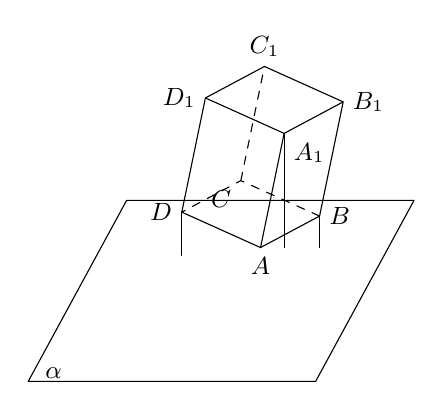
\begin{tikzpicture}[line cap=round,line join=round,font=\small]
  \coordinate (A)  at (1.25,0.35);
  \coordinate (B)  at (2.00,0.75);
  \coordinate (C)  at (1.00,1.20);
  \coordinate (D)  at (0.25,0.80);
  \coordinate (A1) at (1.55,1.80);
  \coordinate (B1) at (2.30,2.20);
  \coordinate (C1) at (1.30,2.65);
  \coordinate (D1) at (0.55,2.25);

  % 平面 α：A 位于其上，边界按源图作透视示意。
  \draw (-0.45,0.95)--(3.20,0.95)--(1.95,-1.35)--(-1.70,-1.35)--cycle;

  % 立方体可见棱与遮挡棱。
  \draw (D)--(A)--(B);
  \draw[dashed] (B)--(C)--(D);
  \draw (D)--(D1) (A)--(A1) (B)--(B1);
  \draw[dashed] (C)--(C1);
  \draw (D1)--(C1)--(B1)--(A1)--cycle;

  % 相邻顶点到平面 α 的距离线，仅作源图中的位置示意，不标尺寸。
  \draw[thin] (D)--(0.25,0.25);
  \draw[thin] (B)--(2.00,0.35);
  \draw[thin] (A1)--(1.55,0.35);

  \node[below] at (A) {$A$};
  \node[right] at (B) {$B$};
  \node[below left] at (C) {$C$};
  \node[left] at (D) {$D$};
  \node[below right] at (A1) {$A_1$};
  \node[right] at (B1) {$B_1$};
  \node[above] at (C1) {$C_1$};
  \node[left] at (D1) {$D_1$};
  \node[below left] at (-1.15,-1.05) {$\alpha$};
\end{tikzpicture}
\end{center}
\nopagebreak[4]
\end{question}
\gkpart{三、解答题}

\begin{question}
\gkti{17}已知 $\dfrac{3\pi}{4}<\alpha<\pi$，$\tan\alpha+\cot\alpha=-\dfrac{10}{3}$。

（1） 求 $\tan\alpha$ 的值；

\Needspace{5\baselineskip}
（2） 求
\nopagebreak[4]
\[
\dfrac{5\sin^2\dfrac{\alpha}{2}+8\sin\dfrac{\alpha}{2}\cos\dfrac{\alpha}{2}+11\cos^2\dfrac{\alpha}{2}-8}{\sqrt{2}\sin\left(\alpha-\dfrac{\pi}{2}\right)}
\]
的值。

\end{question}
\begin{question}
\gkti{18}在添加剂的搭配适用中，为了找到最佳的搭配方案，需要对各种不同的搭配方式作比较。在试制某种牙膏新品种时，需要选用两种不同的添加剂。现有芳香度分别为 $0,1,2,3,4,5$ 的六种添加剂可供选用。根据实验设计学原理，通常首先要随机选取两种不同的添加剂进行搭配实验。用 $\xi$ 表示所选用的两种不同的添加剂的芳香度之和。

（1） 写出 $\xi$ 的分布列；（以列表的形式给出结论，不必写计算过程）

（2） 求 $\xi$ 的数学期望 $E\xi$。（要求写出计算过程或说明道理）

\Needspace{0.4\textheight}
\end{question}
\begin{question}
\gkti{19}如图，$P$ 是边长为 $1$ 的正六边形 $ABCDEF$ 所在平面外一点，$PA=1$，$P$ 在平面 $ABC$ 内的射影为 $BF$ 的中点 $O$。

（1） 证明：$PA\perp BF$；

（2） 求面 $APB$ 与面 $DPB$ 所成二面角的大小。
\nopagebreak[4]
\begin{center}% 2006 安徽卷理 Q19；正六边形及空间点的仿射投影示意，O 为 BF 中点。
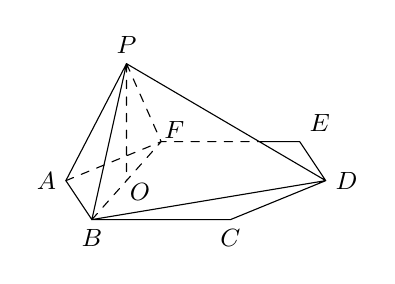
\begin{tikzpicture}[scale=1.1,line cap=round,line join=round,font=\small]
  \coordinate (A) at (0,0);
  \coordinate (B) at (0.3,-0.45);
  \coordinate (C) at (1.9,-0.45);
  \coordinate (D) at (3,0);
  \coordinate (E) at (2.7,0.45);
  \coordinate (F) at (1.1,0.45);
  \coordinate (H) at (2.2333333,0.45); % PD 与 FE 的图示交点，仅用于分段绘线
  \coordinate (O) at (0.7,0);
  \coordinate (P) at (0.7,1.35);

  \draw[dashed] (A)--(F)--(H) (B)--(F) (P)--(F) (P)--(O);
  \draw (H)--(E) (A)--(B)--(C)--(D)--(E) (B)--(D) (P)--(A) (P)--(B) (P)--(D);

  \node[left] at (A) {$A$};
  \node[below] at (B) {$B$};
  \node[below] at (C) {$C$};
  \node[right] at (D) {$D$};
  \node[above right] at (E) {$E$};
  \node[above right,inner sep=1pt] at (F) {$F$};
  \node[below right,inner sep=1pt] at (O) {$O$};
  \node[above] at (P) {$P$};
\end{tikzpicture}
\end{center}
\nopagebreak[4]
\end{question}
\begin{question}
\gkti{20}已知函数 $f(x)$ 在 $\mathbb R$ 上有定义，对任意实数 $a>0$ 和任意实数 $x$，都有
\nopagebreak[4]
\[
f(ax)=af(x)\text{。}
\]

（1） 证明 $f(0)=0$；

\Needspace{5\baselineskip}
（2） 证明
\nopagebreak[4]
\[
f(x)=\begin{cases}
kx,&x\geqslant0,\\
hx,&x<0,
\end{cases}
\]
其中 $k$ 和 $h$ 均为常数；

（3） 当（2）中的 $k>0$ 时，设 $g(x)=\dfrac{1}{f(x)}+f(x)$（$x>0$），讨论 $g(x)$ 在 $(0,+\infty)$ 内的单调性并求极值。

\end{question}
\begin{question}
\gkti{21}数列 $\{a_n\}$ 的前 $n$ 项和为 $S_n$，已知 $a_1=\dfrac12$，$S_n=n^2a_n-n(n-1)$，$n=1,2,\ldots$。

（1） 写出 $S_n$ 与 $S_{n-1}$ 的递推关系式（$n\geqslant2$），并求 $S_n$ 关于 $n$ 的表达式；

（2） 设 $f_n(x)=\dfrac{S_n}{n}x^{n+1}$，$b_n=f_n'(p)$（$p\in\mathbb R$），求数列 $\{b_n\}$ 的前 $n$ 项和 $T_n$。

\Needspace{0.4\textheight}
\end{question}
\begin{question}
\gkti{22}如图，$F$ 为双曲线 $C\text{：}\dfrac{x^2}{a^2}-\dfrac{y^2}{b^2}=1$（$a>0,b>0$）的右焦点，$P$ 为双曲线 $C$ 右支上一点，且位于 $x$ 轴上方，$M$ 为左准线上一点，$O$ 为坐标原点。已知四边形 $OFPM$ 为平行四边形，$|PF|=\lambda|OF|$。

（1） 写出双曲线 $C$ 的离心率 $e$ 与 $\lambda$ 的关系式；

（2） 当 $\lambda=1$ 时，经过焦点 $F$ 且平行于 $OP$ 的直线交双曲线于 $A,B$ 点，若 $|AB|=12$，求此时的双曲线方程。
\nopagebreak[4]
\begin{center}% 2006 安徽卷理 Q22；取 a=1、e=2 作满足题设几何关系的示意。
\begin{tikzpicture}[x=0.9cm,y=0.72cm,line cap=round,line join=round,>=stealth,font=\small]
  \coordinate (O) at (0,0);
  \coordinate (F) at (2,0);
  \coordinate (M) at (-0.5,{sqrt(15)/2});
  \coordinate (P) at (1.5,{sqrt(15)/2});
  \draw[->] (-3.4,0)--(3.5,0) node[right] {$x$};
  \draw[->] (0,-3.7)--(0,3.9) node[above] {$y$};
  \draw (-0.5,-3.1)--(-0.5,3.1);
  \draw[thick,domain=-3.4:3.4,samples=100] plot ({sqrt(1+\x*\x/3)},\x);
  \draw[thick,domain=-3.4:3.4,samples=100] plot ({-sqrt(1+\x*\x/3)},\x);
  \draw (O)--(M)--(P)--(F);
  \node[below right] at (O) {$O$};
  \node[below] at (F) {$F$};
  \node[left] at (M) {$M$};
  \node[above left] at (P) {$P$};
\end{tikzpicture}
\end{center}
\nopagebreak[4]

\end{question}